\subsection{Résultats des simulations par la méthode des éléments finis (\acrshort{FEM})}

Après avoir déterminé les différents paramètres liés à la géométrie et à l'import des composants dans Patran, 
il est temps de réaliser les différents tests de résistance et de fréquence de résonance des pièces afin de 
confirmer mécaniquement nos réalisations.

\subsubsection{Validation de la tenue mécanique de la pièce principale de séparation}
Pour débuter notre étude, focalisons-nous sur la pièce mécanique en aluminium 7075-T6 située entre le tube du 
premier étage et le système de connexion du second étage. Cette pièce doit résister à la fois aux efforts 
axiaux lors du vol et aux efforts en flexion horizontale.

\begin{figure}[h!]
    \centering
    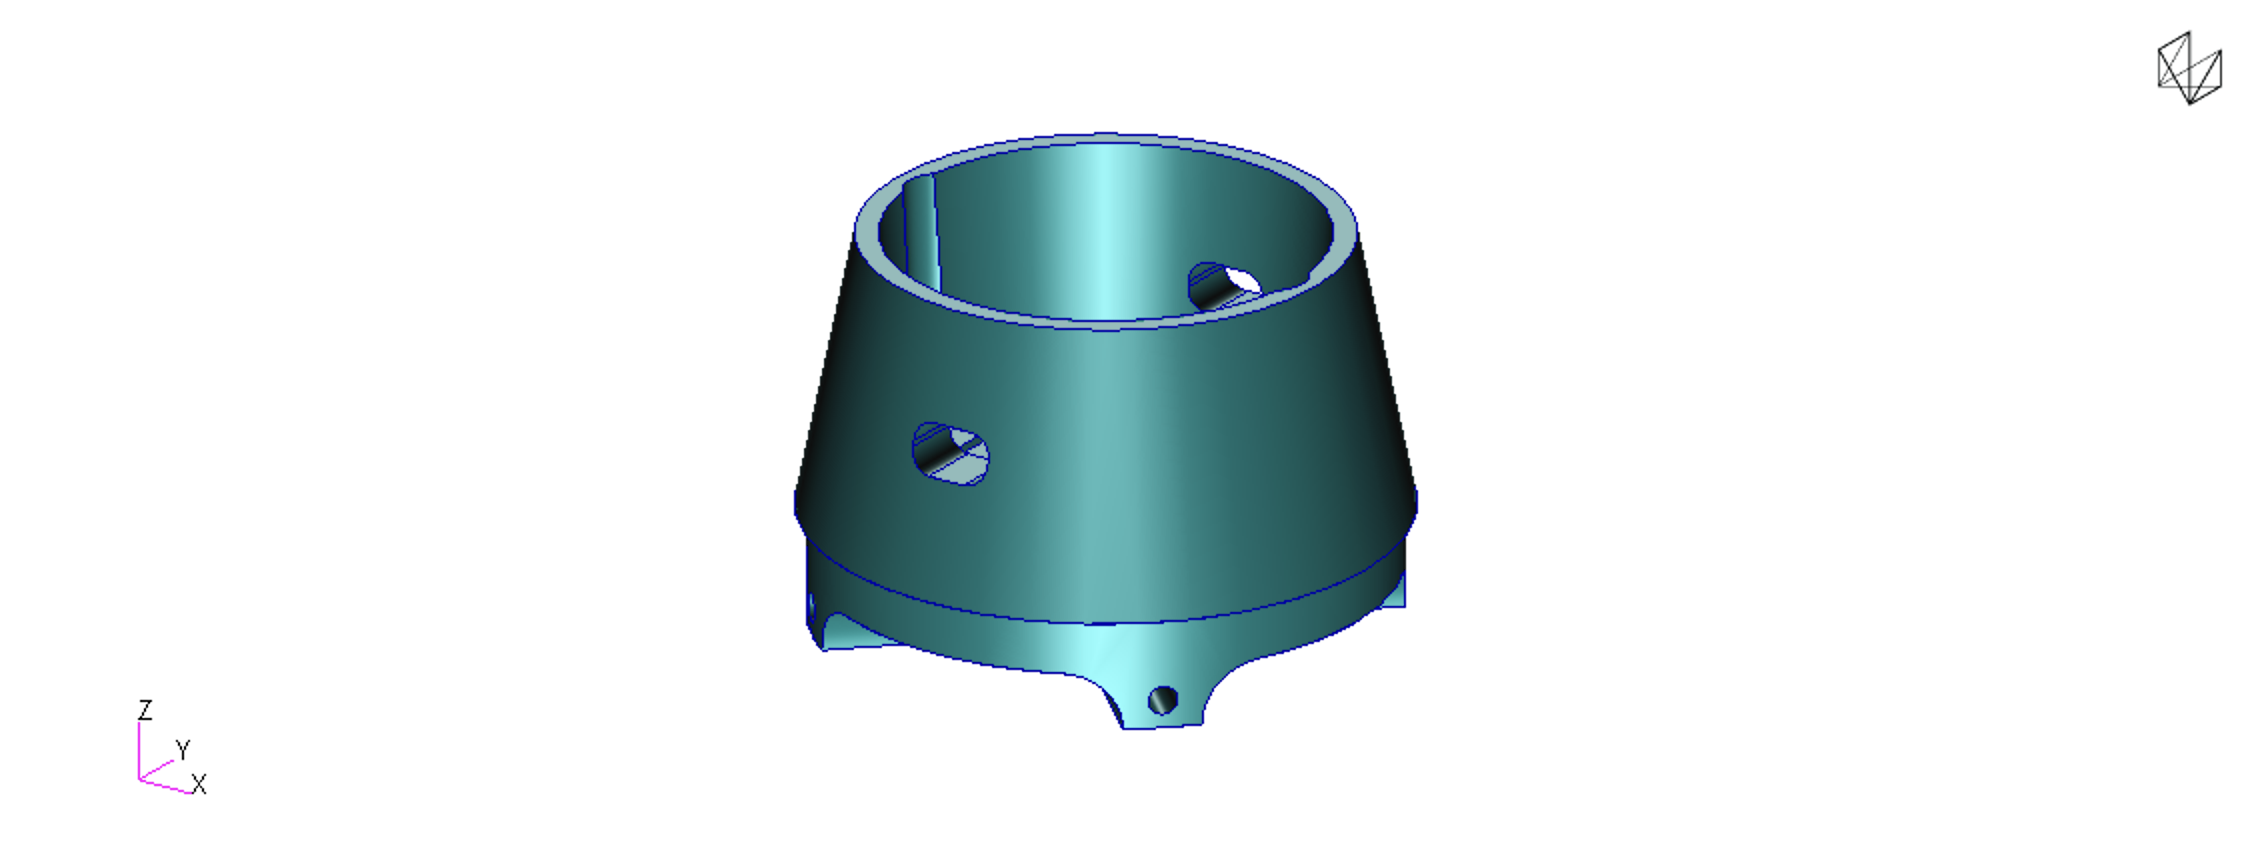
\includegraphics[width=1\linewidth]{figures/visu_import_patran.png}
    \caption{Pièce de séparation du premier étage}
    \label{fig:piece_separation}
\end{figure}

L'application des contraintes d'encastrement au niveau des quatre vis M5 et de la contrainte liée au tube en 
fibre de verre permet de limiter le mouvement de la pièce à une rotation autour de l'axe Z, sans translation. 
Une charge totale ("Total load") a été appliquée pour simuler la déformation de la pièce sous l'influence de 
la masse de la fusée au décollage, avec un facteur de sécurité de 1,5. Cette charge est répartie sur la surface 
plane supérieure et, de manière moins importante, sur la surface conique reliant les deux étages.

L'analyse statique linéaire (SOL-101) nous permet d'évaluer les déformations maximales et les contraintes de 
von Mises dans la pièce. Les résultats sont présentés ci-dessous :

\begin{itemize}
    \item \textbf{Déformée maximale} : D'après les Figures \ref{fig:displacement1} et \ref{fig:displacement2}, 
    la déformation maximale observée est de \textbf{2,04 mm}. Cette valeur reste acceptable pour une pièce en 
    aluminium 7075-T6, dont la limite élastique est d'environ 500 MPa. Les zones les plus sollicitées se situent 
    autour des encastrements et de la surface conique, ce qui est cohérent avec les efforts appliqués.
\end{itemize}

\begin{figure}[h!]
    \centering
    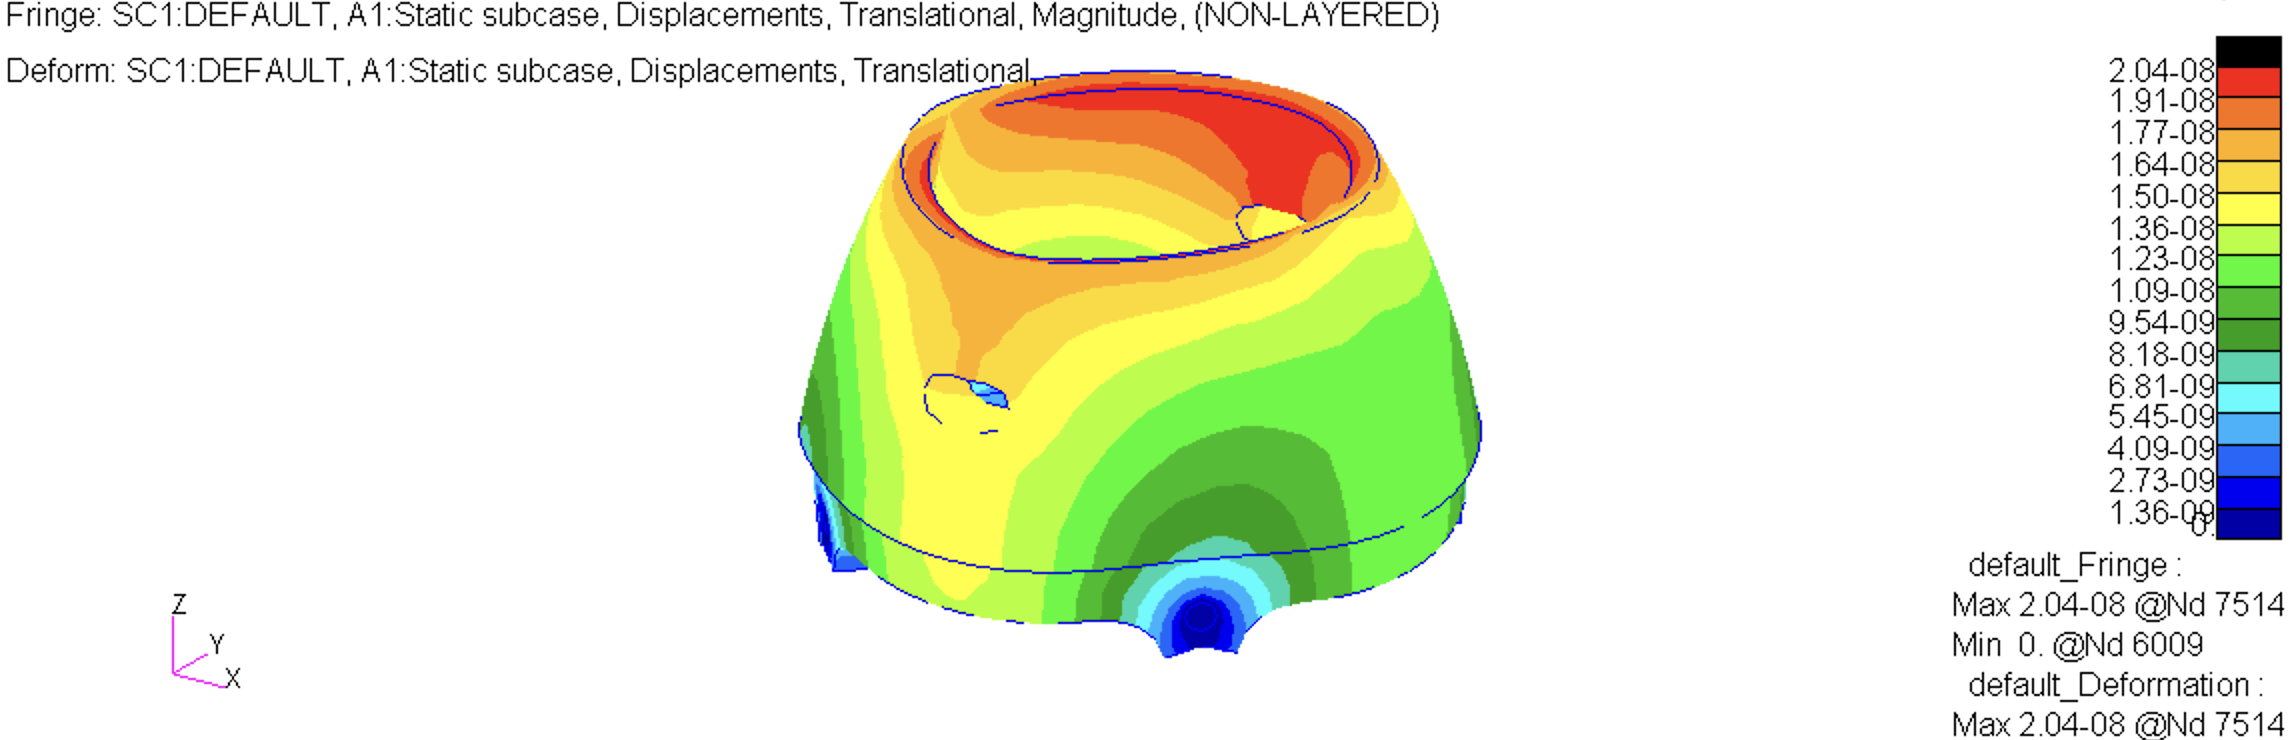
\includegraphics[width=1\linewidth]{figures/displacements_translational1.png}
    \caption{Visualisation de la déformée maximale de la pièce de séparation du premier étage}
    \label{fig:displacement1}
\end{figure}

\begin{figure}[h!]
    \centering
    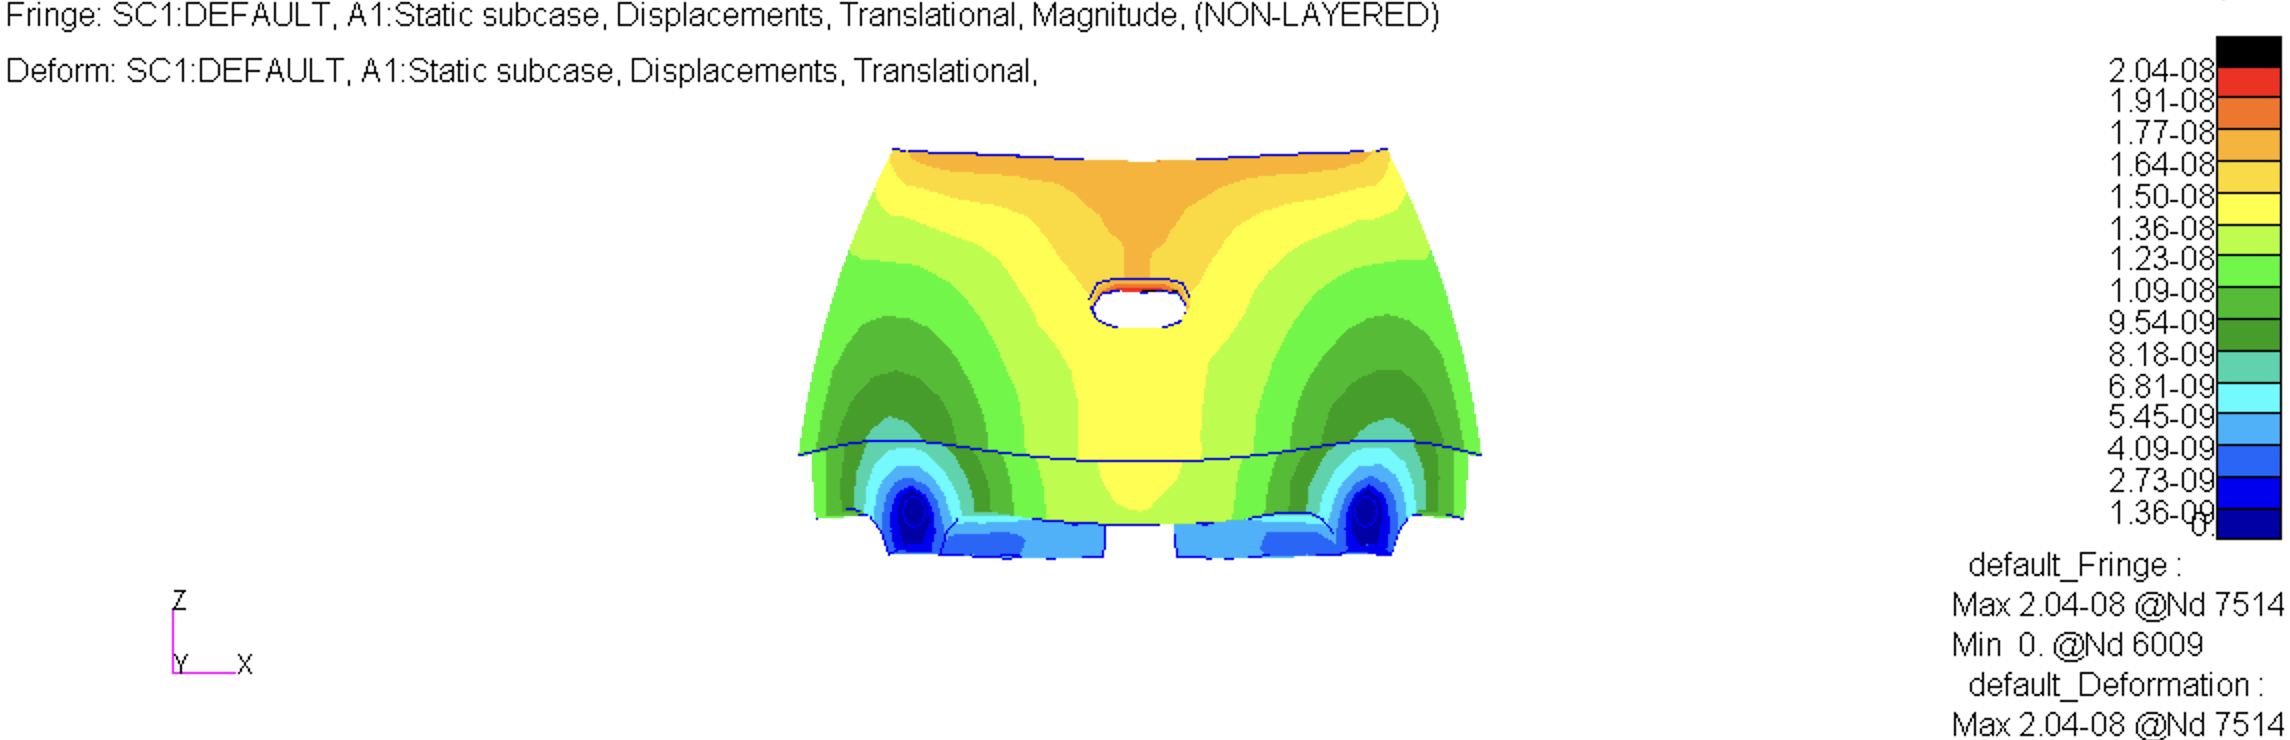
\includegraphics[width=1\linewidth]{figures/displacements_tranlational2.png}
    \caption{Visualisation de la contrainte maximale de la pièce de séparation du premier étage}
    \label{fig:displacement2}
\end{figure}


\begin{itemize}
    \item \textbf{Contrainte maximale} : La Figure \ref{fig:stress_tensor} 
    montre que la contrainte maximale atteint environ \textbf{600 MPa}. Cette valeur dépasse 
    légèrement la limite élastique théorique de l'alliage 7075-T6 (500 MPa), ce qui suggère 
    une nécessité de renforcement local ou une révision des contraintes appliquées. Cependant, 
    cette contrainte maximale est localisée et ne remet pas en cause l'intégrité globale de la pièce.
\end{itemize}

\begin{figure}[h!]
    \centering
    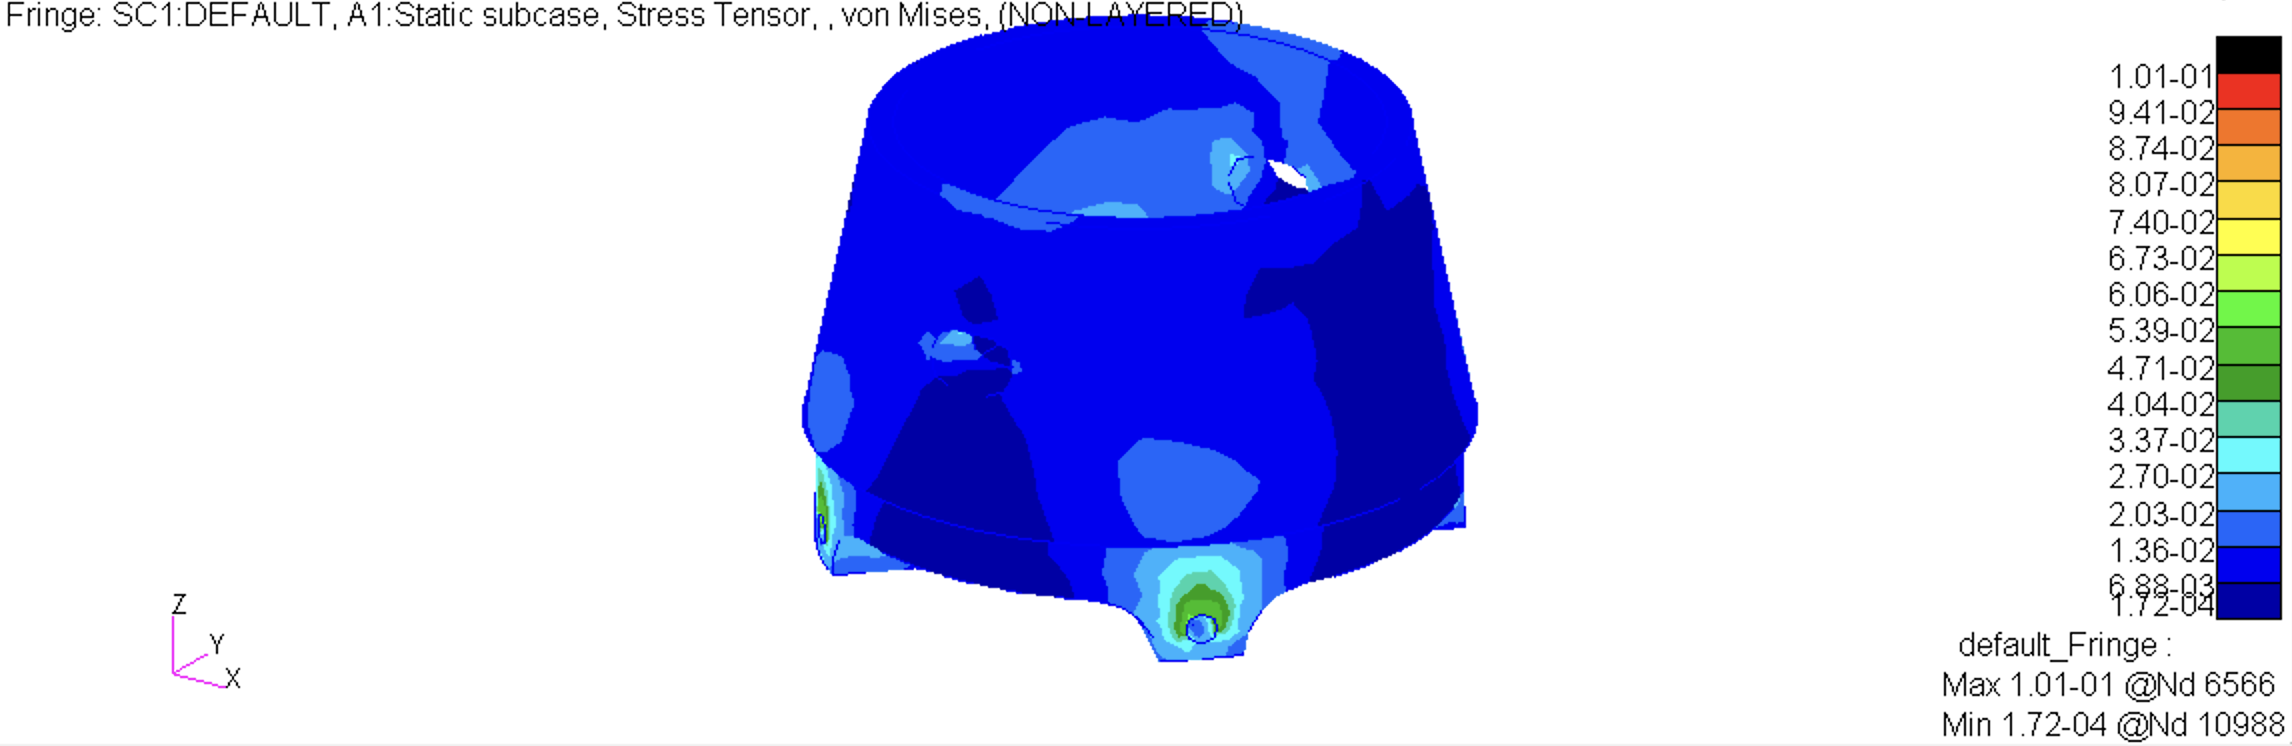
\includegraphics[width=1\linewidth]{figures/stress_tensor.png}
    \caption{Contraintes de von Mises sur la pièce de séparation du premier étage}
    \label{fig:stress_tensor}
\end{figure}

Étant donné que cette pièce n'atteint pas des valeurs critiques de contrainte maximale aux endroits critiques, 
trous de vis, trous et poches... nous pouvons la considérer analytiquement rigide pour de futures analyses.


\subsubsection{Analyse modale d'une pièce en aluminium}
L'analyse modale rélalisée permet également de valider les problèmes de résonance en série dans des assemblages complexes.
Cette partie nous permtet de nous familiariser avec la méthode de résolution de Patran SOL-103. Ici, nous représentons la 
première fréquence de résonance en pièce libre sans contrainte pour mieux comprendre visuellement.
\begin{figure}[h!]
    \centering
    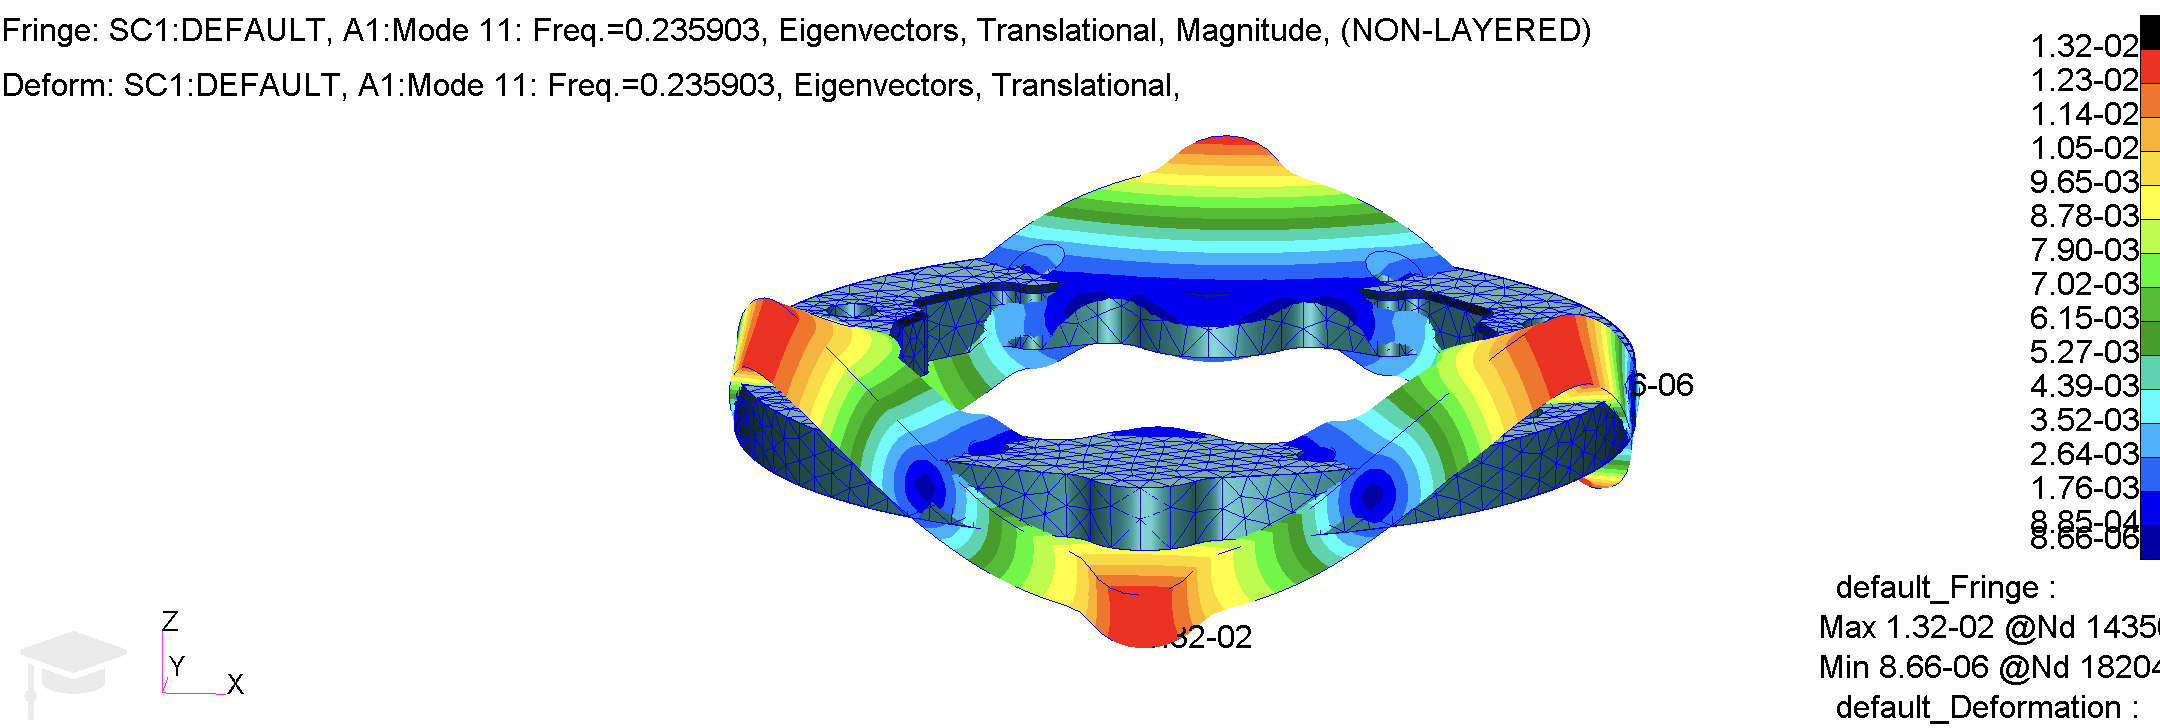
\includegraphics[width=0.8\linewidth]{figures/analyse_modale.png}
    \caption{Analyse modale (fréquences de résonance)}
    \label{fig:resonance}
\end{figure}




\newpage
\subsubsection{Analyse des loquets}
Les loquets, conçus pour maintenir la connexion entre les étages, ont également été simulés sous charge.
En effet, ces derniers sont soumis à différents types de contraintes. Sur le diamètre principal, une rotation type rotule 
(sans translation sur l'axe) est possible, et un encastrement est défini sur le trou inférieur, lié à son maintien avec la vis 
sans fin dans l'aaseblage principal.
Enfin, dans les études ralisées, la configuration 1 loquet a été retunu pour simplifier le temps de calcul, ce qui requiert 
l'application de la force pour un seul des loquets dans cette configuration.\\
\begin{figure}[h!]
    \centering
    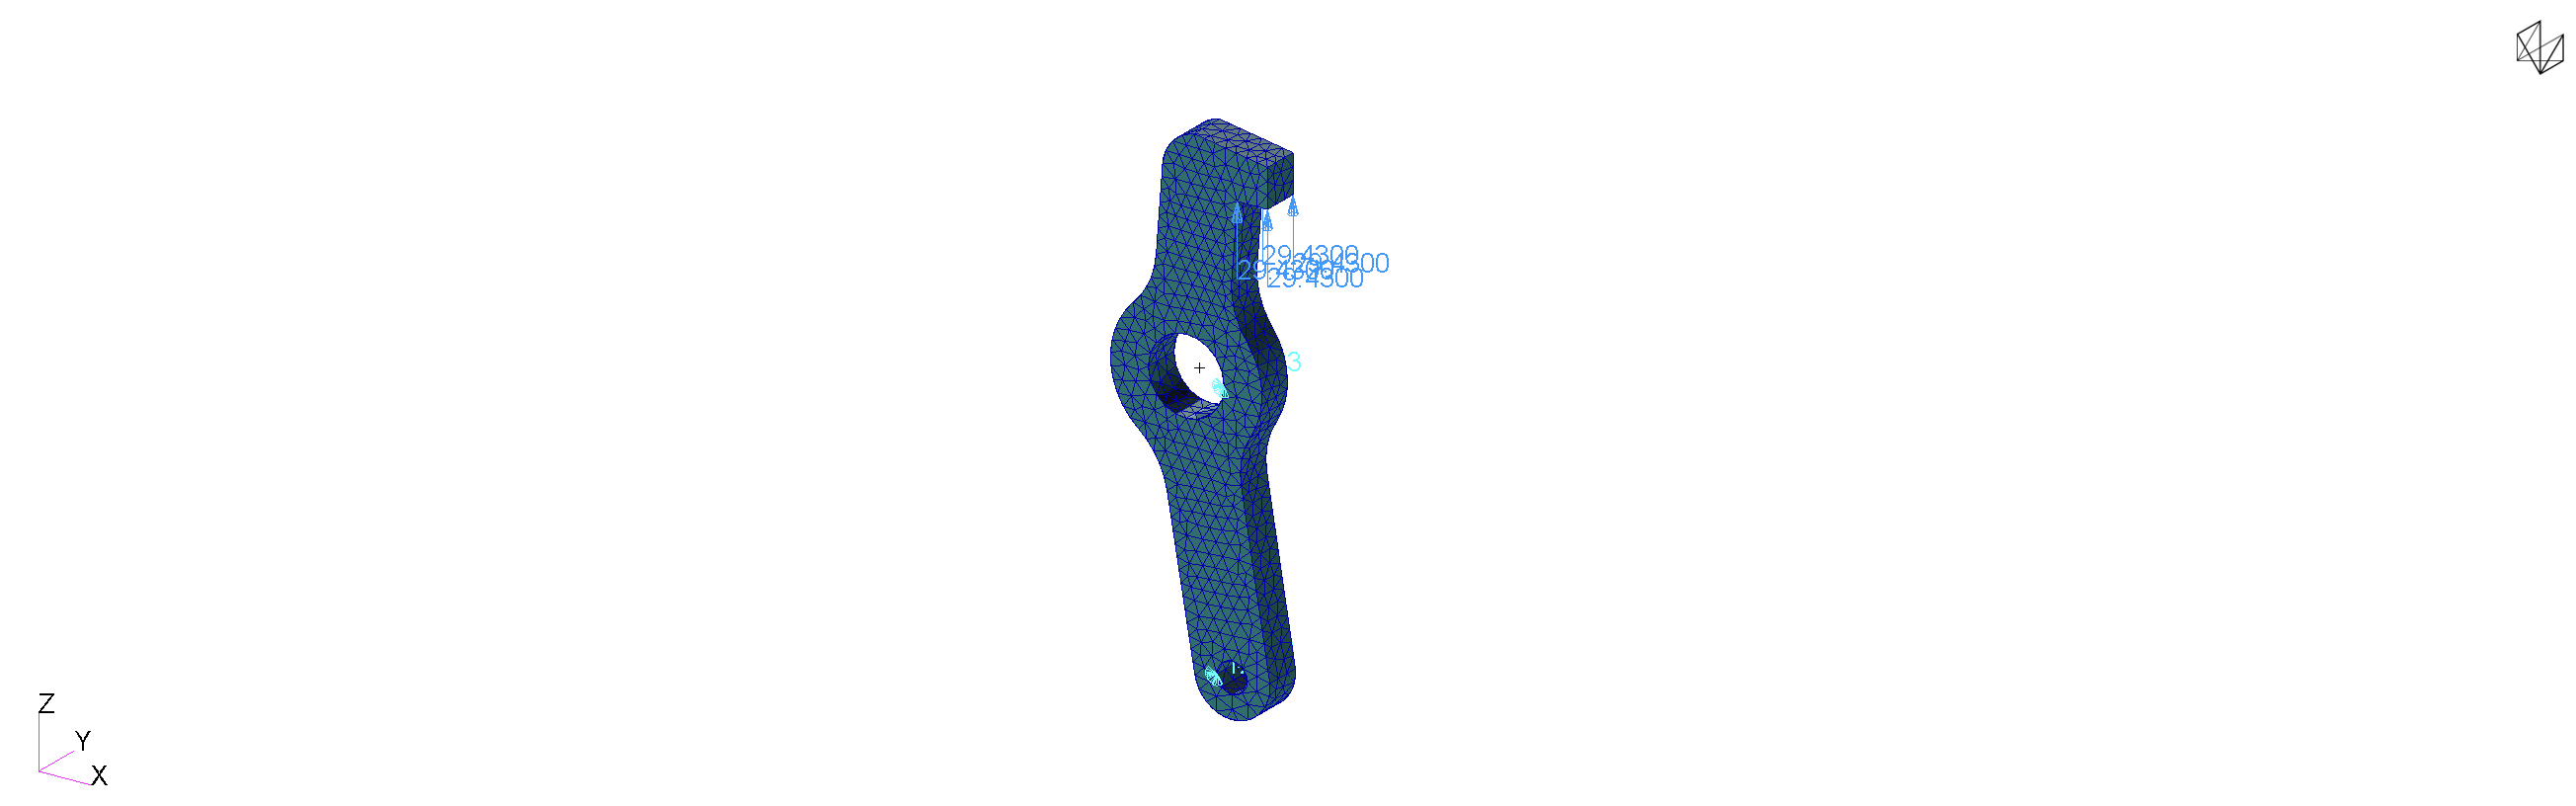
\includegraphics[width=1\linewidth]{figures/LOQUET_force.png}
    \caption{Design d'un loquet avec contraintes appliquées}
    \label{fig:loquet_design}
\end{figure}

Les résultats sont les suivants :

\begin{itemize}
    \item \textbf{Déformée maximale} (Figure \ref{fig:displacement_loquet}) : La déformation maximale 
    observée est de \textbf{0,525E-8 mm}, ce qui est bien acceptable pour un mécanisme de verrouillage, 
    à condition que cette déformation n'affecte pas la fonctionnalité du système.
\end{itemize}

\begin{figure}[h!]
    \centering
    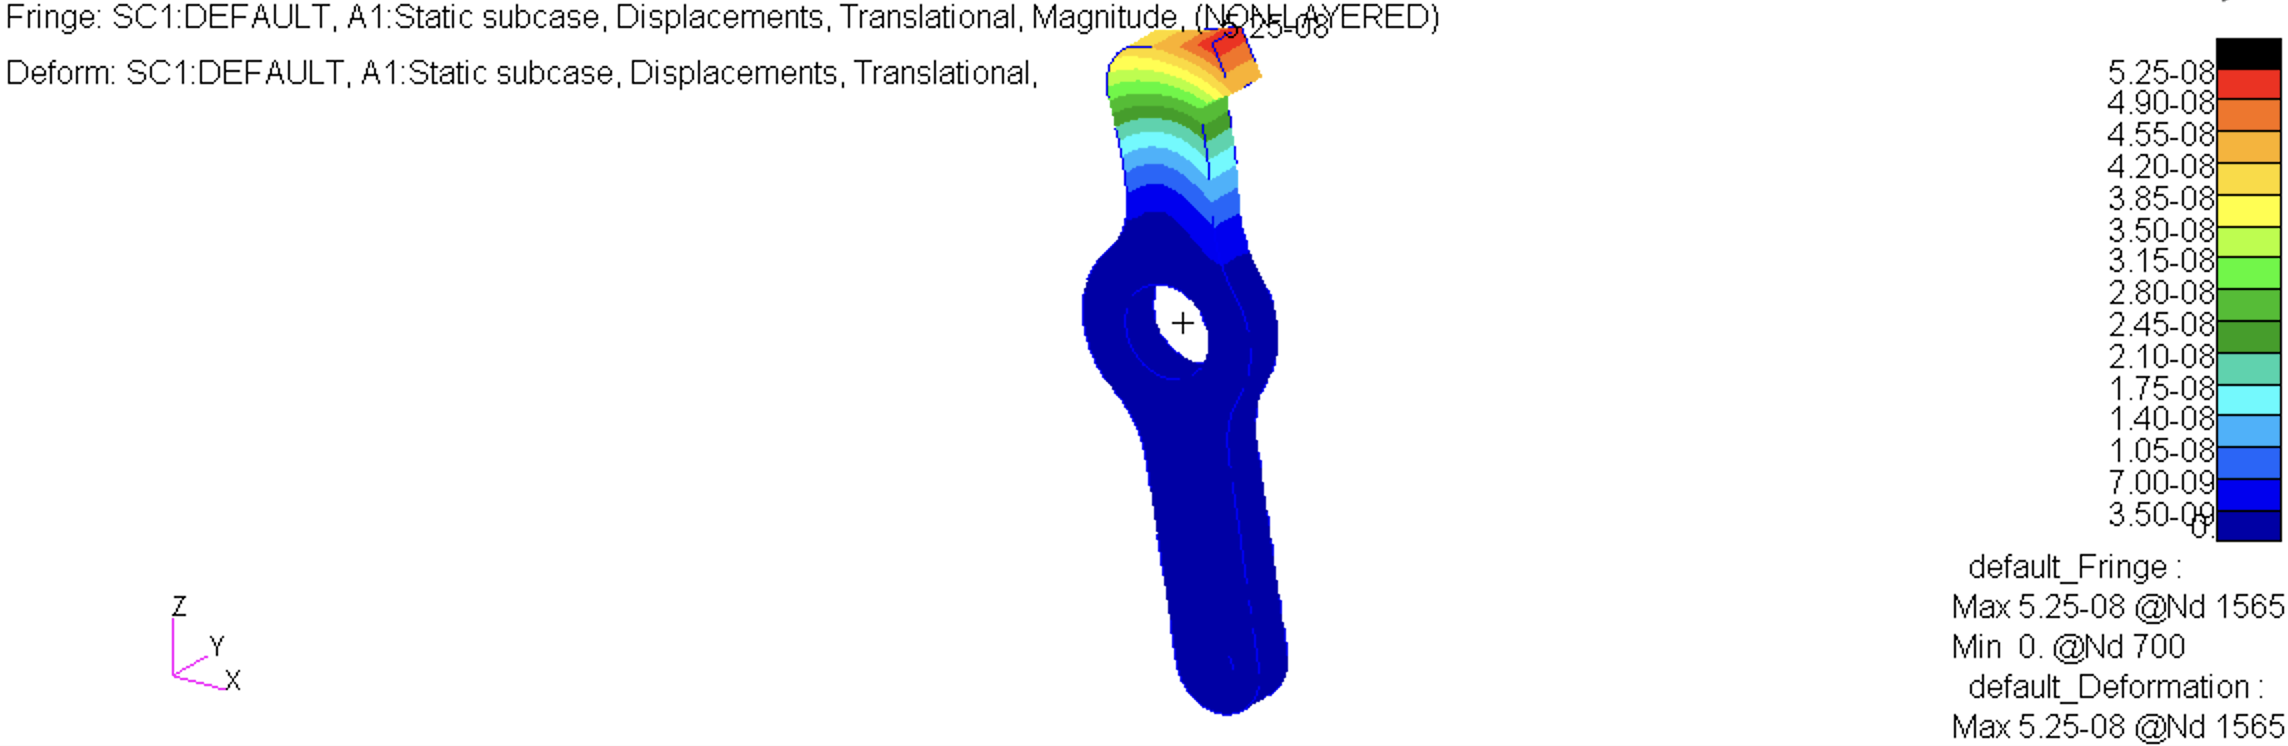
\includegraphics[width=0.8\linewidth]{figures/displacements_loquet.png}
    \caption{Déformée maximale sur un loquet avec contraintes appliquées}
    \label{fig:displacement_loquet}
\end{figure}

\begin{itemize}
    \item \textbf{Contrainte maximale} (Figure \ref{fig:stress_loquet}) : Les contraintes maximales 
    atteignent environ \textbf{0,525 MPa} dans les zones critiques. Cette valeur est élevée mais reste acceptable
    dans la configration d'un crochet en aluminium 7075-T6. Toutefois, la représentation montre les endroits succeptibles
    de subir des défaillances sur le long terme dans ces zones.
\end{itemize}

\begin{figure}[h!]
    \centering
    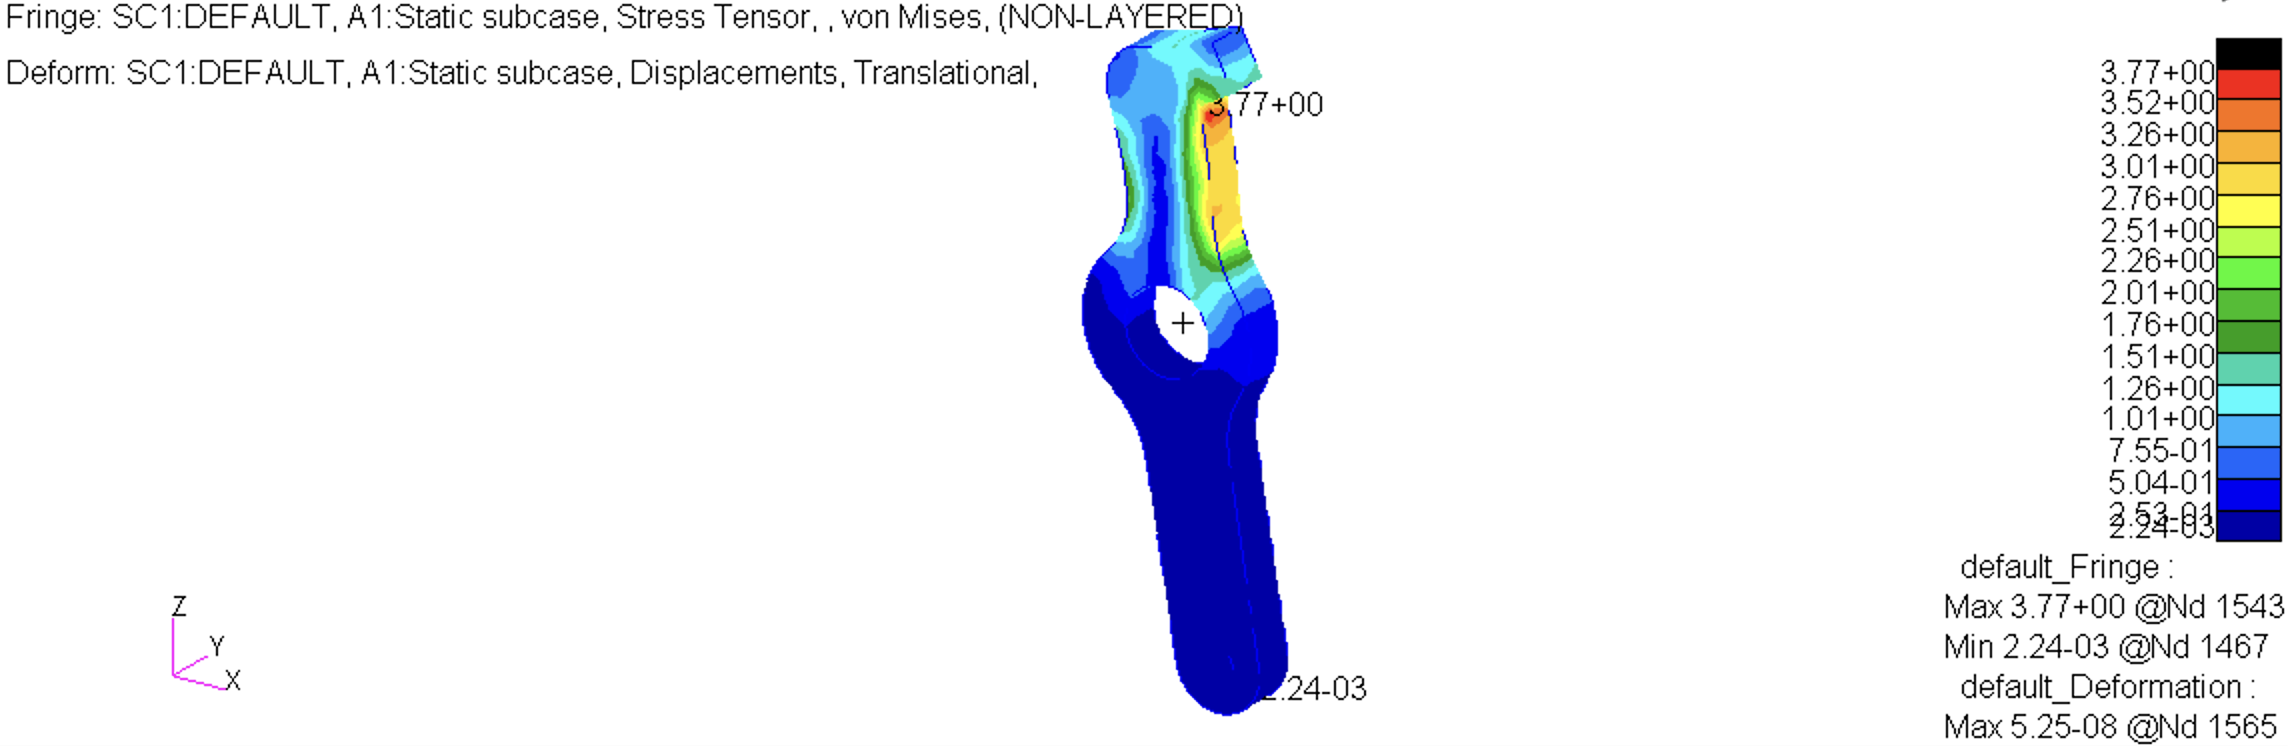
\includegraphics[width=0.8\linewidth]{figures/stress_loquet.png}
    \caption{Contraintes de von Mises sur un loquet avec contraintes appliquées}
    \label{fig:stress_loquet}
\end{figure}

\newpage
\newpage
\subsection{Comparaison des résultats analytiques et numériques}

Dans cette section, nous comparons les résultats obtenus par des méthodes analytiques avec ceux issus des simulations réalisées dans Patran. Cette comparaison permet de valider les modèles numériques et d'identifier les écarts éventuels.

\subsubsection{Analyse de la pièce de séparation}

\subsubsubsection{Calcul analytique de la déformée maximale}

Pour une pièce soumise à une charge uniformément répartie, la déformée maximale peut être estimée analytiquement en utilisant la théorie des plaques ou des poutres, selon la géométrie. Pour une plaque circulaire encastrée soumise à une pression uniforme \(p\), la déformée maximale \(w_{\text{max}}\) au centre est donnée par :

\[
w_{\text{max}} = \frac{p R^4}{64 D}
\]

où \(R\) est le rayon de la plaque, et \(D\) est la rigidité flexionnelle définie par :

\[
D = \frac{E h^3}{12(1 - \nu^2)}
\]

avec \(E\) le module de Young, \(h\) l'épaisseur de la plaque, et \(\nu\) le coefficient de Poisson.

\subsubsubsection*{Application numérique :}
Pour notre pièce de séparation en aluminium 7075-T6 (\(E = 71,7 \, \text{GPa}\), \(\nu = 0,33\)), avec une épaisseur pour modélier la secrion supérieure la plus sollicitée \(h = 5 \, \text{mm}\) et un rayon \(R = 100 \, \text{mm}\), soumise à une pression \(p = 1 \, \text{MPa}\) :

\[
D = \frac{71,7 \times 10^9 \times (5 \times 10^{-3})^3}{12(1 - 0,33^2)} = 76,3 \, \text{Nm}
\]

\[
w_{\text{max}} = \frac{1 \times 10^6 \times (0,1)^4}{64 \times 76,3} = 0,26 \, \text{mm}
\]

\subsubsubsection{Résultats Patran}

Les simulations réalisées dans Patran montrent une déformée maximale de \(2,04 \, \text{mm}\) (voir Figure \ref{fig:displacement1}). Cette différence peut s'expliquer par plusieurs facteurs :
- La géométrie réelle de la pièce n'est pas une plaque circulaire parfaite.
- Les conditions aux limites dans Patran incluent des encastrements localisés (vis M5), ce qui modifie la répartition des contraintes.
- La charge appliquée dans Patran n'est pas uniformément répartie.

\subsubsubsection{Comparaison et discussion}

\begin{table}[h!]
    \centering
    \caption{Comparaison des déformées maximales}
    \begin{tabular}{|c|c|c|}
    \hline
    & \textbf{Analytique} & \textbf{Patran} \\
    \hline
    Déformée maximale & \(0,26 \, \text{mm}\) & \(2,04 \, \text{mm}\) \\
    \hline
    \end{tabular}
    \label{tab:deformee_comparaison}
\end{table}

La différence entre les résultats analytiques et numériques souligne l'importance de la modélisation précise des conditions aux limites et de la géométrie réelle dans les simulations numériques.


\subsubsection{Analyse des loquets}

\subsubsubsection{Calcul analytique de la déformée}

Pour une poutre encastrée soumise à une force ponctuelle \(F\) à son extrémité, la déformée maximale \(w_{\text{max}}\) est donnée par :

\[
w_{\text{max}} = \frac{F L^3}{3 E I}
\]

où \(L\) est la longueur de la poutre, \(E\) le module de Young, et \(I\) le moment d'inertie.

\subsubsubsection*{Application numérique :}
Pour un loquet en aluminium 7075-T6 (\(E = 71,7 \, \text{GPa}\)), avec une longueur \(L = 50 \, \text{mm}\), une section rectangulaire de \(10 \times 5 \, \text{mm}\), et une force \(F = 30xk_{safety} \, \text{N}\) pour 4 loquets :

\[
I = \frac{b h^3}{12} = \frac{10 \times 10^{-3} \times (5 \times 10^{-3})^3}{12} = 1,04 \times 10^{-11} \, \text{m}^4
\]

\[
w_{\text{max}} = \frac{\frac{30\times 1,5}{4} \times (0,05)^3}{3 \times 71,7 \times 10^9 \times 1,04 \times 10^{-11}} = 0,45 \, \text{mm}
\]

Cette valeur permet de nous rendre compte de la déformée pour une longueur de 50mm, et dans le cas de notre géométrie usinée, nous aurons 6mm d'aluminium en contact, au lieu du 50mm calculé. Cela rejoindra la valeur obenue sur Patran.
Les simulations Patran montrent une déformée maximale de \(5,25E-8 \, \text{mm}\) (voir Figure \ref{fig:displacement_loquet}).



\newpage
\subsubsection{Analyse des pièces en composite}
Pour les pièces en composite, les propriétés mécaniques sont déterminées à l'aide des lois de mélange et 
des modèles semi-empiriques comme Halpin-Tsai.

\subsubsubsection{Lois de mélange pour les composites}
Afin de déterminer le module longitudinal \(E_{11}\), nous utilisons la loi de mélange suivante :
\[
E_{11} = V_f E_f + (1 - V_f) E_m
\]

Pour déterminer le module transverse \(E_T\), nous utilisons le modèle semi-empirique de Halpin-Tsai :
\[
\frac{E_T}{E_m} = \frac{1 + \xi \eta V_f}{1 - \eta V_f}, \quad \text{où} \quad \eta = \frac{(E_f/E_m) - 1}{(E_f/E_m) + \xi}
\]

\subsubsubsection{Module de cisaillement et coefficient de Poisson}
Le module de cisaillement \(G_{LT}\) est déterminé par la règle inverse des mélanges :
\[
\frac{1}{G_{LT}} = \frac{V_f}{G_f} + \frac{V_m}{G_m}
\]

Le coefficient de Poisson \(\nu_{LT}\) est calculé comme suit :
\[
\nu_{LT} = \nu_f V_f + \nu_m V_m
\]
La relation entre les coefficients de Poisson et les modules est donnée par :
\[
\frac{\nu_{LT}}{E_L} = \frac{\nu_{TL}}{E_T}
\]

\begin{figure}[h!]
    \centering
    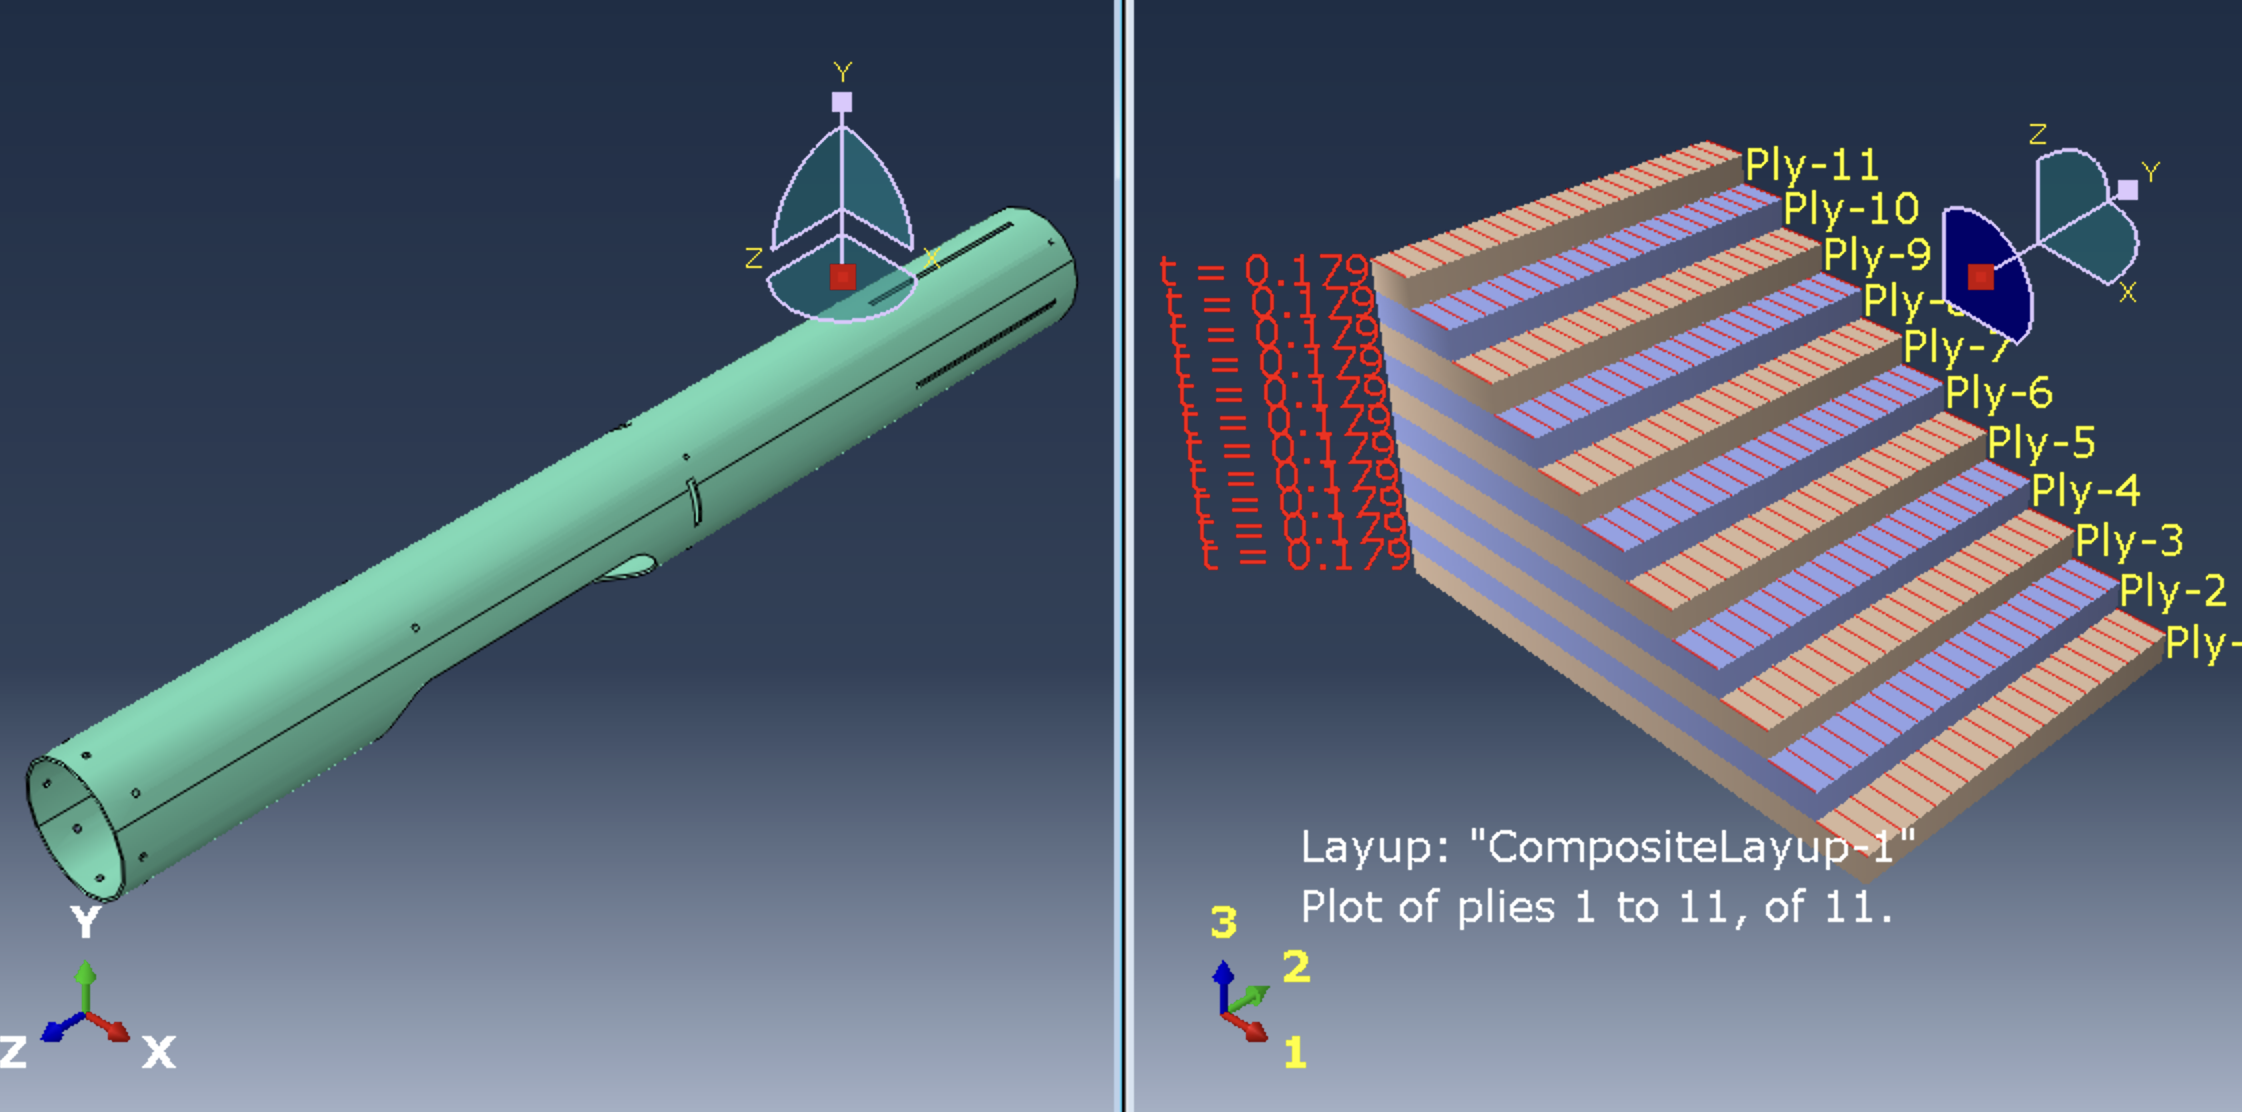
\includegraphics[width=0.8\linewidth]{figures/simu_composite.png}
    \caption{Définition du composite du tube porteur du premier étage}
    \label{fig:stress_loquet}
\end{figure}

La validation du matériel a été faite avec un échantillon à Abaqus pour valider la structure qui reliera notre moduléparation au vecteur de propulsion.


\newpage